\begin{figure}
	\centering
	\begin{minipage}[b]{.5\linewidth}
		\centering
		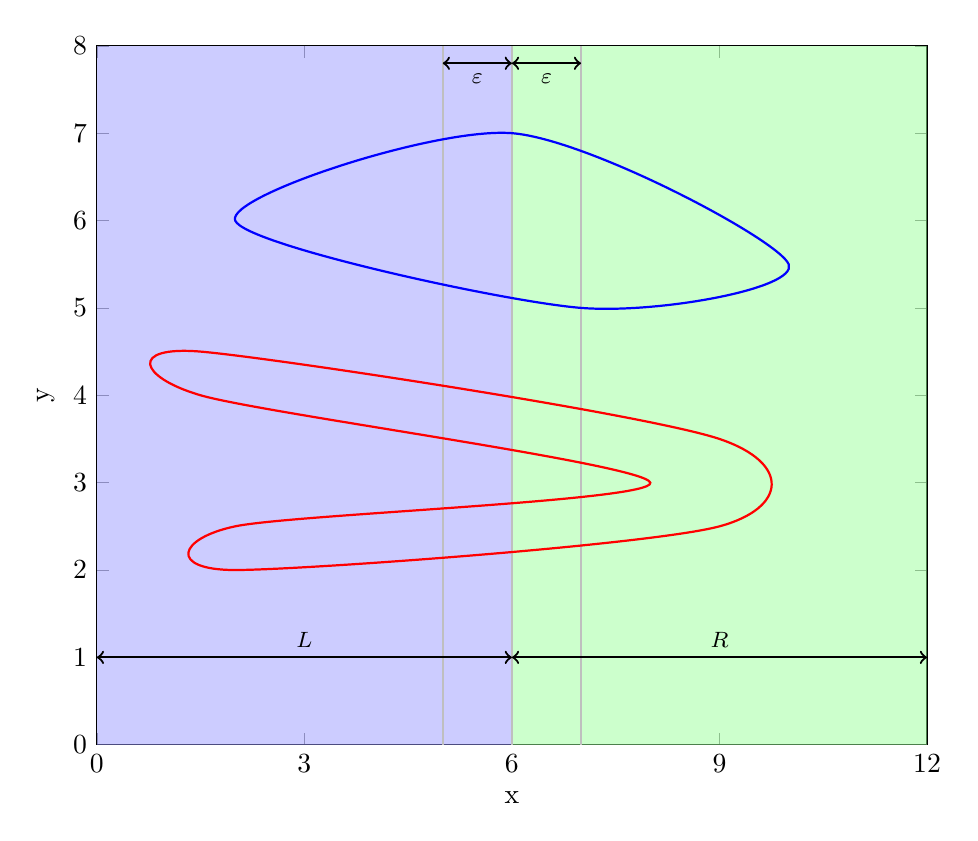
\begin{tikzpicture}
		\begin{axis}[
		width=\linewidth,
		xlabel=x, ylabel=y,
		xmin=0, ymin=0, xmax=12, ymax=8,
		xtick={0,3,6,9,12}
		]
		
		\filldraw[fill=blue!40, draw=none, opacity=.5] (0,0) rectangle (6,8);
		\filldraw[fill=green!40, draw=none, opacity=.5] (6,0) rectangle (12,8);
				
		\def \mydraw{\draw[font=\footnotesize,thick,<->]}
		
		\draw[gray!50,thick] (5,0) -- ++(0,8);
		\draw[gray!50,thick] (6,0) -- ++(0,8);
		\draw[gray!50,thick] (7,0) -- ++(0,8);
		\mydraw (5,7.8) -- node[below] {$ \varepsilon $} ++(1,0);
		\mydraw (6,7.8) -- node[below] {$ \varepsilon $} ++(1,0);
		
		\mydraw (0,1) --  node[above] {$ L $} ++(6,0);				
		\mydraw (6,1) -- node[above] {$ R $} ++(6,0);	
		
		\draw [blue, thick] plot [smooth cycle] coordinates {(2,6) (6, 7) (10, 5.5) (7, 5)};
		\draw [red, thick] plot [smooth cycle] coordinates {(1.5,4) (1.5,4.5) (9, 3.5) (9, 2.5)  (2, 2) (2, 2.5) (8, 3)};
		\end{axis}
		\end{tikzpicture}
		\subcaption{grupy odkryte w zbiorze $ D $}\label{qscan:partitioned-clusters-D}
	\end{minipage}%
	\begin{minipage}[b]{.5\linewidth}
		\centering
		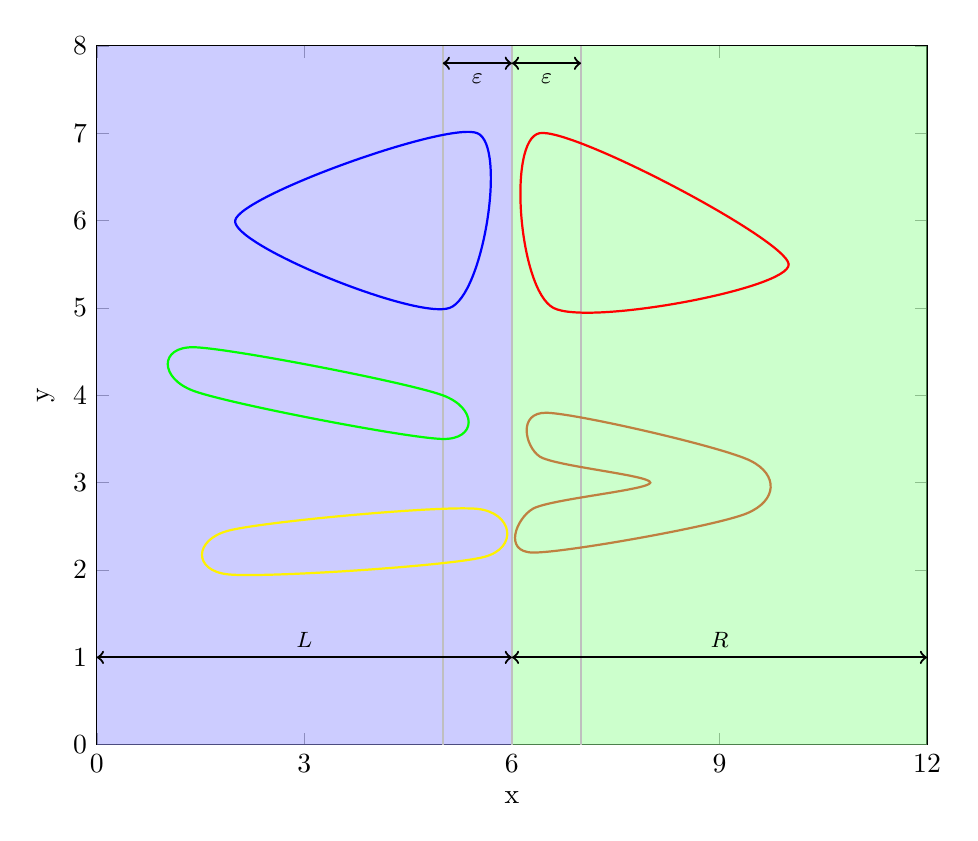
\begin{tikzpicture}
		\begin{axis}[
		width=\linewidth,
		xlabel=x, ylabel=y,
		xmin=0, ymin=0, xmax=12, ymax=8,
		xtick={0,3,6,9,12}
		]
		
		\filldraw[fill=blue!40, draw=none, opacity=.5] (0,0) rectangle (6,8);
		\filldraw[fill=green!40, draw=none, opacity=.5] (6,0) rectangle (12,8);
		
		\def \mydraw{\draw[font=\footnotesize,thick,<->]}
		
		\draw[gray!50,thick] (5,0) -- ++(0,8);
		\draw[gray!50,thick] (6,0) -- ++(0,8);
		\draw[gray!50,thick] (7,0) -- ++(0,8);
		\mydraw (5,7.8) -- node[below] {$ \varepsilon $} ++(1,0);
		\mydraw (6,7.8) -- node[below] {$ \varepsilon $} ++(1,0);
		
		\mydraw (0,1) --  node[above] {$ L $} ++(6,0);				
		\mydraw (6,1) -- node[above] {$ R $} ++(6,0);	
		
		\draw [blue, thick] plot [smooth cycle] coordinates {(2,6) (5.5, 7) (5.1, 5)};
		\draw [red, thick] plot [smooth cycle] coordinates {(6.4, 7) (10, 5.5) (6.6, 5)};
		
		\draw [green, thick] plot [smooth cycle] coordinates {(1.4,4.05) (1.4,4.55) (5,4) (5,3.5)};
		\draw [brown, thick] plot [smooth cycle] coordinates {(6.5,3.8) (9.45, 3.25) (9.4, 2.65) (6.3,2.2) (6.3,2.7) (8,3) (6.4,3.3)};
		\draw [yellow, thick] plot [smooth cycle] coordinates { (1.9, 1.95) (1.9, 2.45) (5.5,2.7) (5.6,2.15)};

		\end{axis}
		\end{tikzpicture}
		\subcaption{grupy odkryte w zbiorach $ L $, $ R $}\label{qscan:partitioned-clusters-L-R}
	\end{minipage}
	\caption{Przykładowe grupowanie zbioru $ D $ z parametrem $ \varepsilon = 1 $ oraz prawdopodobne grupowanie podzbiorów $ L $ oraz $ R $, dla pozycji granicy podziału $ b=6 $ i wymiarowi granicy podziału $ d=x $.}\label{qscan:partitioned-clusters}
\end{figure}